\documentclass[a4paper]{article}

\usepackage[utf8]{inputenc}
\usepackage[T1]{fontenc}
%\usepackage{mathptmx}
\usepackage{FiraSans}
\usepackage[left=0.5in, right=0.5in, top=0.5in, bottom=1in]{geometry}
\usepackage[skip=12pt, indent=0pt]{parskip}
\usepackage{titling}
\usepackage{graphicx, subcaption}
\usepackage[dvipsnames]{xcolor}
\usepackage[export]{adjustbox}
\usepackage{hyperref}
\usepackage{mathtools}
\usepackage{amssymb}
\usepackage{enumitem}
\usepackage{listings}
\usepackage[framemethod=TikZ]{mdframed}

\definecolor{custom-blue}{RGB}{0,99,166}

\title{VU Grundlagen des experimentellen Arbeitens \\ Haus{\"u}bung Kryptografie}
\author{Christoph Gro{\ss} \\ a01025119}
\date{\today}

\global\mdfdefinestyle{mdstyle}{
backgroundcolor=blue!10   ,%
linecolor=blue!50!black   ,%
linewidth=3pt             ,%
roundcorner=20pt          ,%
innerleftmargin=1cm       ,%
innerrightmargin=1cm      ,%
skipabove=1cm             ,%
skipbelow=1cm
}

\lstdefinestyle{lststyle}{
commentstyle=\color{teal} ,%
keywordstyle=\color{blue} ,%
basicstyle=\ttfamily\small,%
breaklines=true           ,%
numbers=left              ,%
frame=single
}
\lstset{style=lststyle}

\begin{document}

\begin{titlingpage}
  
\includegraphics[trim={1.2cm 2.2cm 1.2cm 2.2cm},width=6cm]{uni.png}
  \par\rule{\textwidth}{0.5pt}
  \begin{center}
  \vspace*{24pt}
  \textbf{\LARGE\thetitle}\\
  \vspace*{24pt}
  \Large\theauthor\\
  \vspace*{24pt}
  \large\thedate
  \end{center}
\end{titlingpage}

\par Das Ziel der Aufgabe, das Lösen einer C{\"a}sar-Verschl{\"u}sselung, wird durch die
folgenden Schritte erreicht:\\
\begin{itemize}
\item H{\"a}ufigkeitsanalyse der Buchstaben im verschl{\"u}sselten Text (Siehe
\textbf{(a)}).
\item Vergleich mit der Buchstaben-Verteilung in der deutschen Sprache (Siehe
\textbf{(b)}).
\item Den h{\"a}ufigsten codierten Buchstaben mit dem deutschen "E"
gleichsetzen und die (auf das Alphabet bezogene) Distanz berechnen.
\item Alle codierten Buchstaben um diese Distanz verschieben um die
Klarnachricht wiederherzustellen.
\end{itemize}

\par Als Hilfestellung, um langwieriges manuelles Z{\"a}hlen zu vermeiden,
wurde ein \texttt{C}-Programm geschrieben (siehe \ref{appA.sec.caesar}).\\ 
Ein sch{\"o}nes Detail ist das Aufscheinen der Verschiebung der Buchstaben als
horizontaler Versatz im Histogramm.\\
\begin{figure}[h]
  \fbox{\begin{subfigure}{0.45\textwidth}
    \centering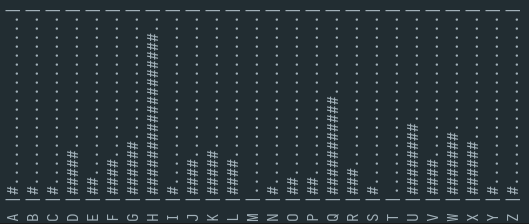
\includegraphics[width=\textwidth]{cesar_letter_dist.png}
    \caption{C{\"a}sar}
    \label{fig1a}
  \end{subfigure}}\quad
  \fbox{\begin{subfigure}{0.45\textwidth}
    \centering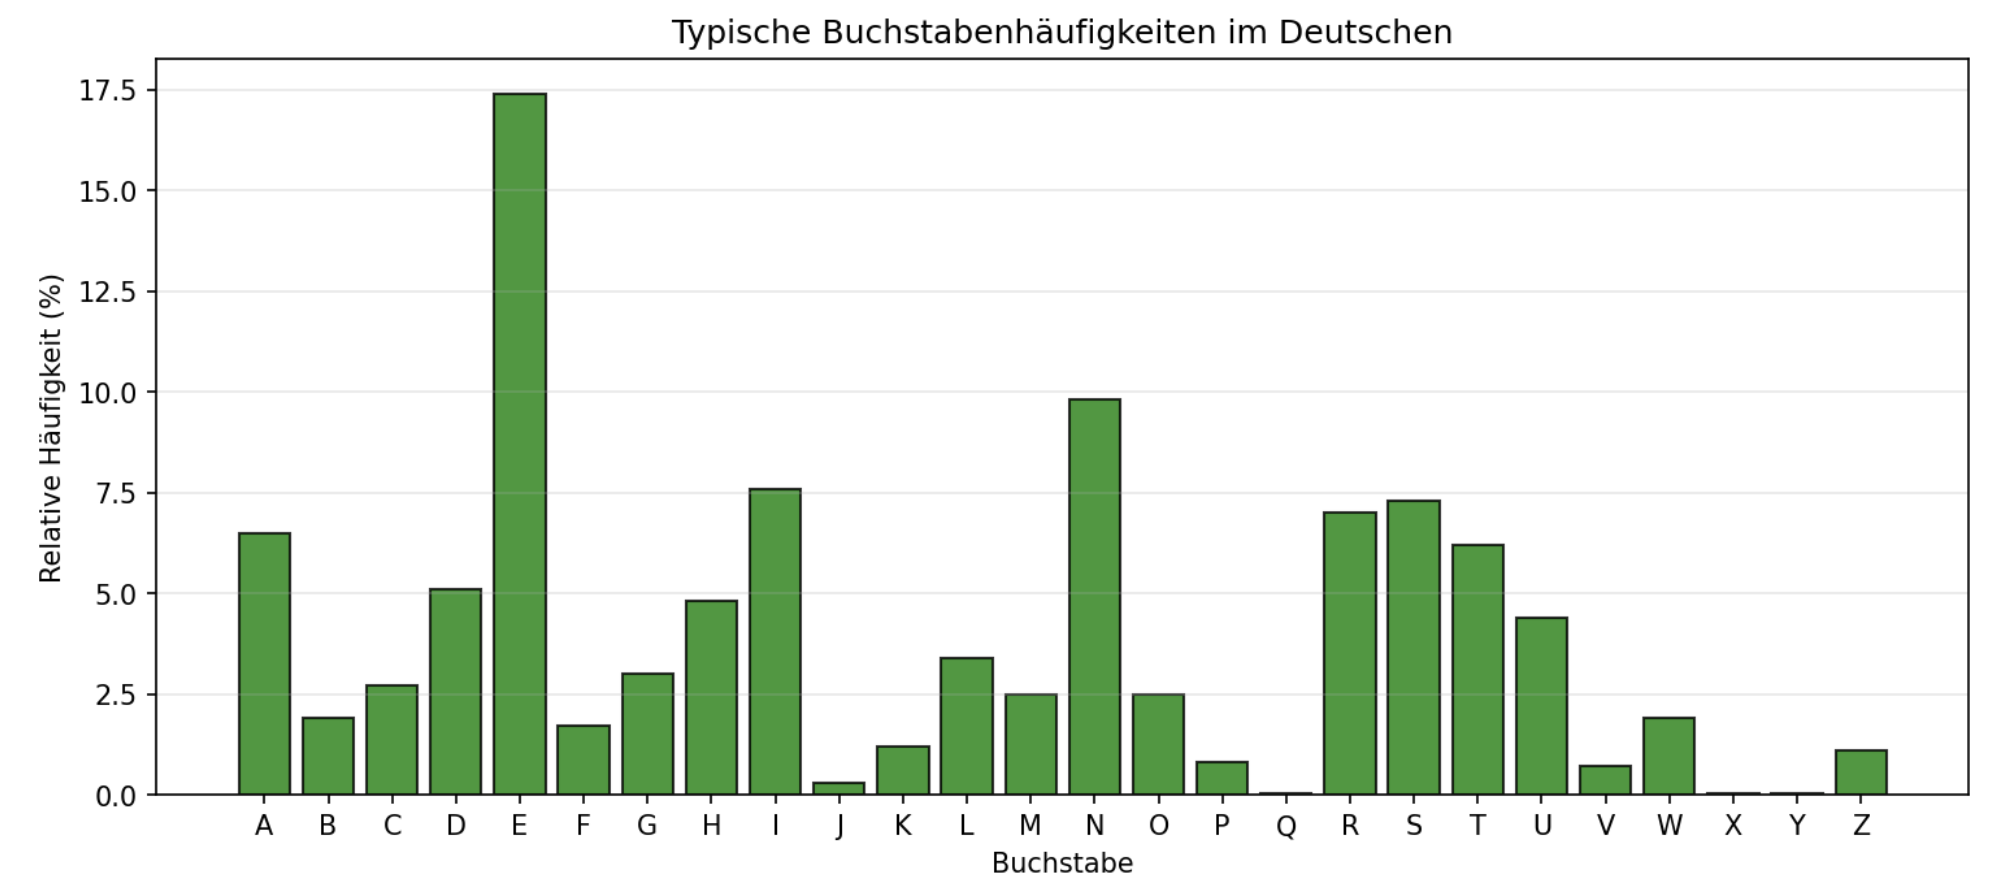
\includegraphics[width=\textwidth]{german_letter_dist.png}
    \caption{Deutsch}
    \label{fig1b}
  \end{subfigure}}
  \end{figure}

\bigskip
\par Dadurch ergibt sich folgende Lösung:

GLH SKBVLN EHVFKUHLEW QDWXUHUVFKHLQXQJHQ GXUFK EHREDFKWXQJHQ HASHULPHQWH XQG PDWKHPDWLVFKH PRGHOOH GXUFK GLH DXVZHUWXQJ YRQ GDWHQ ZHUGHQ JHVHWC XQG UHJHOQ HUNDQQW XQG YRUKHUVDJHQ JHWURIIHQ
\medskip
\begin{center}
$\downarrow$
\end{center}
\medskip
\textcolor{red}{$E \mapsto H \Rightarrow$}
\resizebox{0.9\textwidth}{!}{
\begin{tabular}{ |c|c|c|c|c|c|c|c|c|c|c|c|c|c|c|c|c|c|c|c|c|c|c|c|c|c|} 
 \hline
 A & B & C & D & \textcolor{red}{E} & F & G & H & I & J & K & L & M & N & O & P & Q & R & S & T
 & U & V & W & X & Y & Z \\
 \hline
 D & E & F & G & \textcolor{red}{H} & I & J & K & L & M & N & O & P & Q & R & S & T & U & V & W
 & X & Y & Z & A & B & C \\
 \hline
\end{tabular}}
\medskip
\begin{center}
$\downarrow$
\end{center}
\medskip
DIE PHYSIK BESCHREIBT NATURERSCHEINUNGEN DURCH BEOBACHTUNGEN EXPERIMENTE UND MATHEMATISCHE MODELLE DURCH DIE AUSWERTUNG VON DATEN WERDEN GESETZ UND REGELN ERKANNT UND VORHERSAGEN GETROFFEN
\clearpage

\appendix
\section{Lösungsprogramm \textit{caesar}}
\label{appA.sec.caesar}
\bigskip
\begin{mdframed}[style=mdstyle]
\begin{lstlisting}[language=C, caption=caesar.c]
#include/#defines..

 /* count character occurrences */
  for (int i=0; i<SIZEIN; i++) {
    if (s[i] == '\0') {
      break;
    }   
    if (s[i] >= ASCIIA && s[i] <= ASCIIZ) {
      charDist[s[i]-ASCIIA]++;
      charCnt++;
    }   
  }
  
  /* print distribution */
  char max = printCharDist(charDist, true);
  printCharHist(charDist, charCnt);
  printf("\n Most frequent character: \'%c\'\n", max);
  
  /* shift input by |max - 'E'|%26 */
  int shift = (max - langMaxOcc) % ALPH;

  for (int i=0; i<SIZEIN; i++) {
    if (s[i] == '\0') {
      break;
    }   
    if (s[i] >= ASCIIA && s[i] <= ASCIIZ) {
      s[i] = MODULO(((s[i]-ASCIIA)-shift),ALPH)+ASCIIA;
    }   
  }
\end{lstlisting}
\end{mdframed}

\end{document}
